\documentclass{article}
\usepackage[utf8]{inputenc}
\usepackage{natbib}
\usepackage[french]{babel}
\usepackage{pdfpages}

\title{Rapport du projet de Programmation Système}
\date{\today}

\usepackage{graphicx}
\usepackage[T1]{fontenc}
\usepackage{hyperref} % 		Ajouter des liens
\usepackage{color} % 			Gestion des couleurs
\usepackage[normalem]{ulem} % 	Underline

\usepackage	{comment}%			Commenter

\usepackage	{listingsutf8}% 		Code informatique
\definecolor{mGreen}{rgb}{0,0.6,0}
\definecolor{mGray}{rgb}{0.5,0.5,0.5}
\definecolor{mPurple}{rgb}{0.58,0,0.82}
\definecolor{backgroundColour}{rgb}{0.95,0.95,0.92}
\lstset{
	tabsize=4,
    	extendedchars=true,
    	breaklines=true,
    	keepspaces=true,
	inputencoding=utf8,
    	extendedchars=true,
    	literate=%
                {é}{{\'e}}{1}%
                {è}{{\`e}}{1}%
                {à}{{\`a}}{1}%
                {ç}{{\c{c}}}{1}%
                {œ}{{\oe}}{1}%
                {ù}{{\`u}}{1}%
                {É}{{\'E}}{1}%
                {È}{{\`E}}{1}%
                {À}{{\`A}}{1}%
                {Ç}{{\c{C}}}{1}%
                {Œ}{{\OE}}{1}%
                {Ê}{{\^E}}{1}%
                {ê}{{\^e}}{1}%
                {î}{{\^i}}{1}%
                {ô}{{\^o}}{1}%
                {û}{{\^u}}{1}%
                {ë}{{\¨{e}}}1
                {û}{{\^{u}}}1
                {â}{{\^{a}}}1
                {Â}{{\^{A}}}1
                {Î}{{\^{I}}}1
                {|}{|}1  
}

\lstdefinestyle{NoStyle}{
    language={},
  	backgroundcolor=\color{backgroundColour},
    numberstyle=\tiny\color{mGray},
    basicstyle=\footnotesize,
    numbers=left,
    numbersep=5pt,
  	frame=single,
}

\lstdefinestyle{CMakeStyle}{
    language={},
  	backgroundcolor=\color{backgroundColour},
    numberstyle=\tiny\color{mGray},
    basicstyle=\footnotesize,
    numbers=left,
    numbersep=5pt,
  	frame=single,
}
\lstdefinestyle{C++Style}{
    backgroundcolor=\color{backgroundColour},
    commentstyle=\color{mGreen},
    keywordstyle=\color{magenta},
    numberstyle=\tiny\color{mGray},
    stringstyle=\color{mPurple},
    basicstyle=\footnotesize,
    breakatwhitespace=false,
    breaklines=true,
    captionpos=b,
    numbers=left,
    numbersep=5pt,
    language=C++
}


\begin{document}

\begin{titlepage}
 \begin{sffamily}
  \begin{center}
            
\includegraphics[scale=0.04]{img/ubx-logo.png}
            \\[2cm]
        
    
    {\huge \bfseries Rapport de Projet technologique\\[0.5cm] }

    \rule{\linewidth}{.5pt}
    \\[2cm]

    \begin{minipage}{0.4\textwidth}
      \begin{flushleft} \large
        \author{}Etudiants :\\
        	Marc \textsc{Cerutti}\\
      \end{flushleft}
    \end{minipage}

    \vfill

    {\large \today}

  \end{center}
  \end{sffamily}
  
\end{titlepage}

\newpage

\tableofcontents

%------------------%
\newpage
\part{Présentation du sujet}

\section{Déroulement}
	L'objectif de ce projet de L3 informatique est à terme de créer un robot suiveur qui suivrai son utilisateur à distance de 2 mètres.\\

	On passera cependant par plusieurs étapes.
	\\\\
	D'abord la création de nos fonctions d'analyse ainsi que d'une interface graphique à partir de la bibliothèque OpenCv et Qt respectivement. OpenCv implémente notamment des algorithmes pour faire les filtres, les cartes de disparité et les cartes de profondeur nécessaires à l'analyse d'images pour l'intelligence artificielle, et Qt un système d'interface complet pour pouvoir tester nos fonctions d'analyse d'images.\\
\\\\
	Ensuite la création sous Unity d'une simulation avec les différents paramètres permettant de créer les comportements par défaut du robot et testant les différents algorithmes. Elle devra prévoir les spécificités du matériel et les tests pour différents environnements et situations.\\
	
	Ces deux étapes se feront respectivement au semestre 5 et 6 de Licence informatique 2018-2019.\\
	
\newpage
\section{Analyse de l’existant}

Les consignes sont de s'appuyer sur la bibliothèque d'OpenCv 3.2.0
et Qt supérieur à 4.8 afin d'assurer une compatibilité avec les ordinateurs du Cremi.\\
Du fait de la communauté de OpenCv et de Qt, de nombreux tutoriels sont disponibles en ligne afin de nous permettre d'assurer les fonctionnalités demandé, à savoir l'analyse d'image et la création d'une interface pour tester le résultat.\\
Nous avons aussi comme matériel un robot avec une caméra stéréoscopique mis à la disposition des élèves avec bien sûr des contraintes de disponibilité.

\section{Besoins}

Comme notre programme de traitement d'image sera utilisé dans un système embarqué, la performance de notre code est critique, ainsi que la mémoire utilisé.\\
Il faudra donc pour la portabilité sur le robot exactement savoir les parties de bibliothèque OpenCv à importer.\\
Pour analyser l'environnement du Robot, il faut assurer de la gestion de ces caméra stéréoscopique et le traitement des images qui seront transmis à l'unité de contrôle.\\
Il faudra aussi tester, quantifier les performances, et s'assurer qualitativement du bon déroulement de l'implémentation des fonctionnalités.\\
Il faudra aussi s'assurer de la compatibilité entre le matériel et les bibliothèques.\\

%------------------%
\newpage
\part{Architecture}

\section{Vue Global et conventions}

Il a été choisi pour les fonctions d'analyse d'image de privilégier les fonctions statiques, afin d’être facilement implémentable plus tard dans les algorithmes d'intelligence artificiel. Cela a aussi le mérite de limiter les allouements de mémoires, en ayant en paramètre que ce qui est nécessaire.\\
Cela a cependant des inconvénients au niveau de la maintenabilité en cas de changements de paramètres dans les fonctions, qui peut donc se révéler lourde.\\

Au niveau des dossiers, "tools" rassemble les classes et fonctions concernant le débuguage, la conversion, et le traitement d'images.
Le dossier "subWindows" contient les classes de sous fenêtres à la fenêtre principal de l'interface.\\
La hiérarchie des fichiers est en annexe.\\

La convention de nommage adopté est la suivante :\\

\begin{tabular}{ l c }
   Attribut & \textit{\_name\_complete }\\
   Variables locales  & \textit{name\_complete}\\ 
   Méthodes & \textit{nameComplete}\\
   Classes 	& \textit{NameClass}\\
   Fichiers	& \textit{nameclass.*}\\
 \end{tabular}\\

et la documentation est faite avec doxygen.\\

\newpage
\section{Débogage et performances}

Il faut prévoir le débuguage à la fois sur ordinateur, et sur les robots. C'est pourquoi dans certaines des fonctions, elles peuvent fonctionner sans l'environnement Qt.
Le principal besoin de celles-ci est de permettre un débogage facile, et de calculer les performances des différents algorithmes.\\

Voire la documentation de ProjectUtilities.\\

\newpage
\section{Interface}


L'interface permet à la fois de tester les fonctions implémenté avec leur paramètres que de vérifier qualitativement de la performance des résultats.

La fenêtre principale permet de tester les filtres de base et d'accéder à des sous menus spéciaux en fonction des besoins des développements.\\

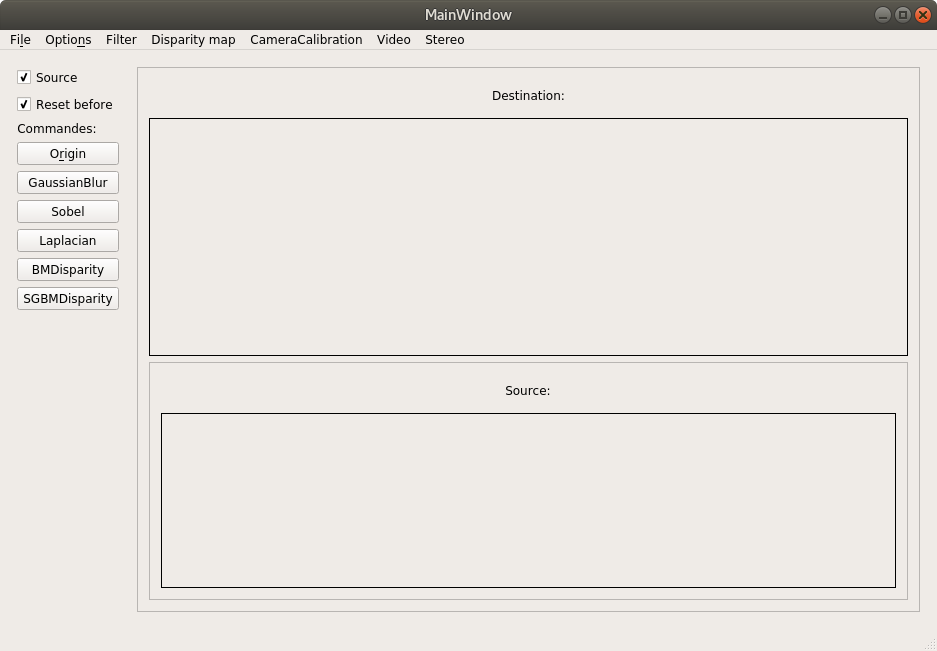
\includegraphics[width=\linewidth]{img/interface.png}

A l'heure actuelle, il y a 3 sous menus, deux pour les tests des algorithmes de carte de disparité, et une pour les tests de calibration de caméra individuelles.\\

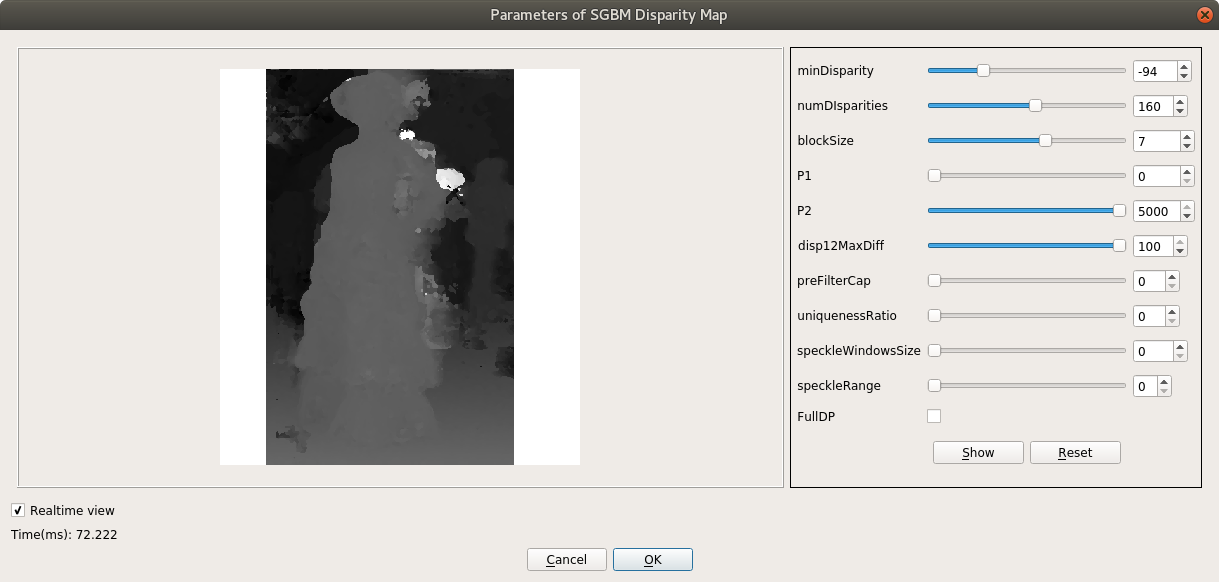
\includegraphics[width=\linewidth]{img/bm.png}\\

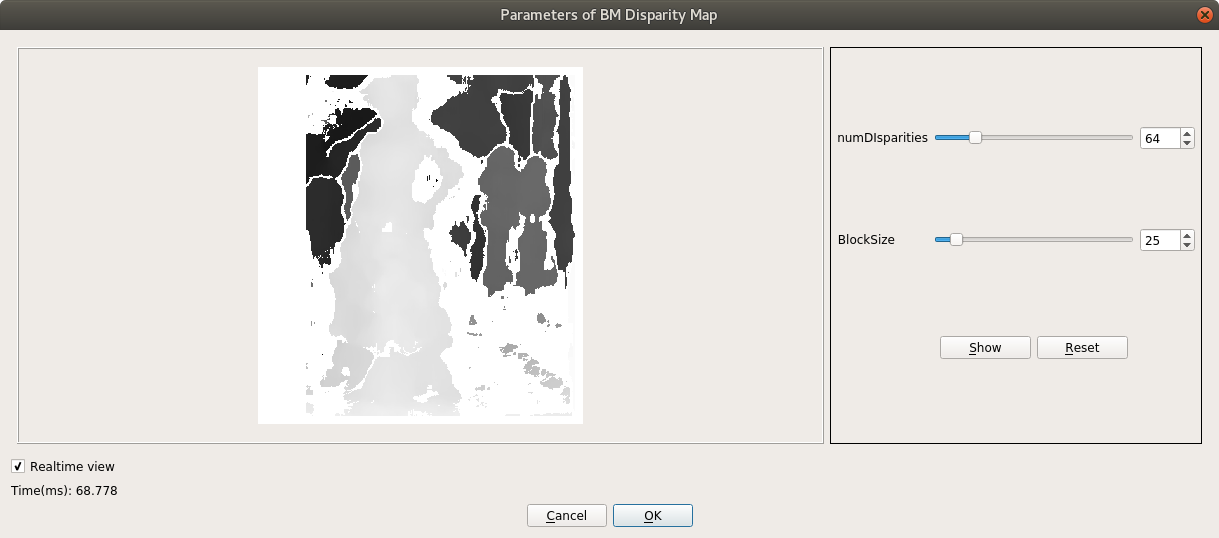
\includegraphics[width=\linewidth]{img/sgbm.png}\\

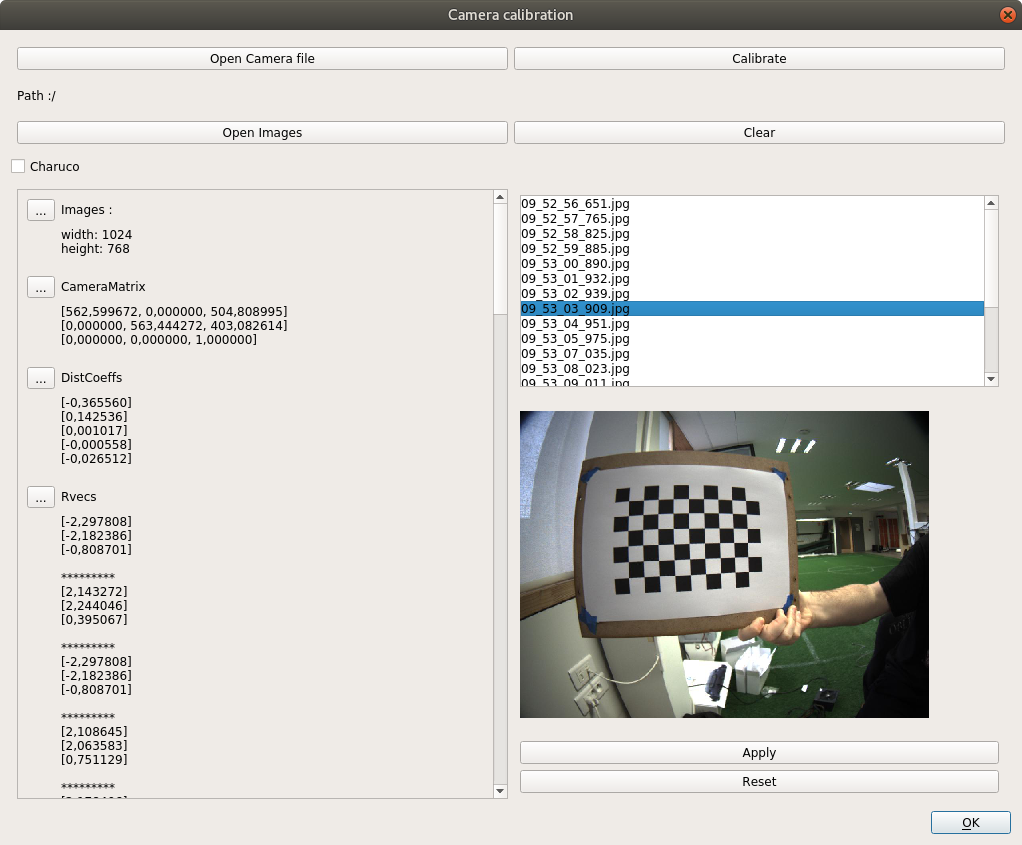
\includegraphics[width=\linewidth]{img/calib.png}\\

Par contre comme les systèmes Qt et OpenCv sur les images ne sont pas compatibles, des fonctions de conversion ont été créé (CVQTInterface).

Une sous-fenêtre pour la calibration stéréo aurait été appréciabl e mais par manque de temps pour l'adaptation d'un système compatible vidéo CV-Qt, et certains problèmes qui seront rappelé dans l'analyse vidéo, un simple système de fenêtre OpenCv pour la visualisation et l'extraction d'image a été implémenté.\\
Le système affiche deux vu simultané avec la vidéo de l’œil gauche et la vidéo de l’œil droit. Avec SPACEBAR nous pouvons accepté les vidéos et un débug s'affiche, ou les rejeter avec ESCAPE.
On peut désactiver le système manuel, setter la frame de début, et le nombre de frame qui peut être optionnel.\\

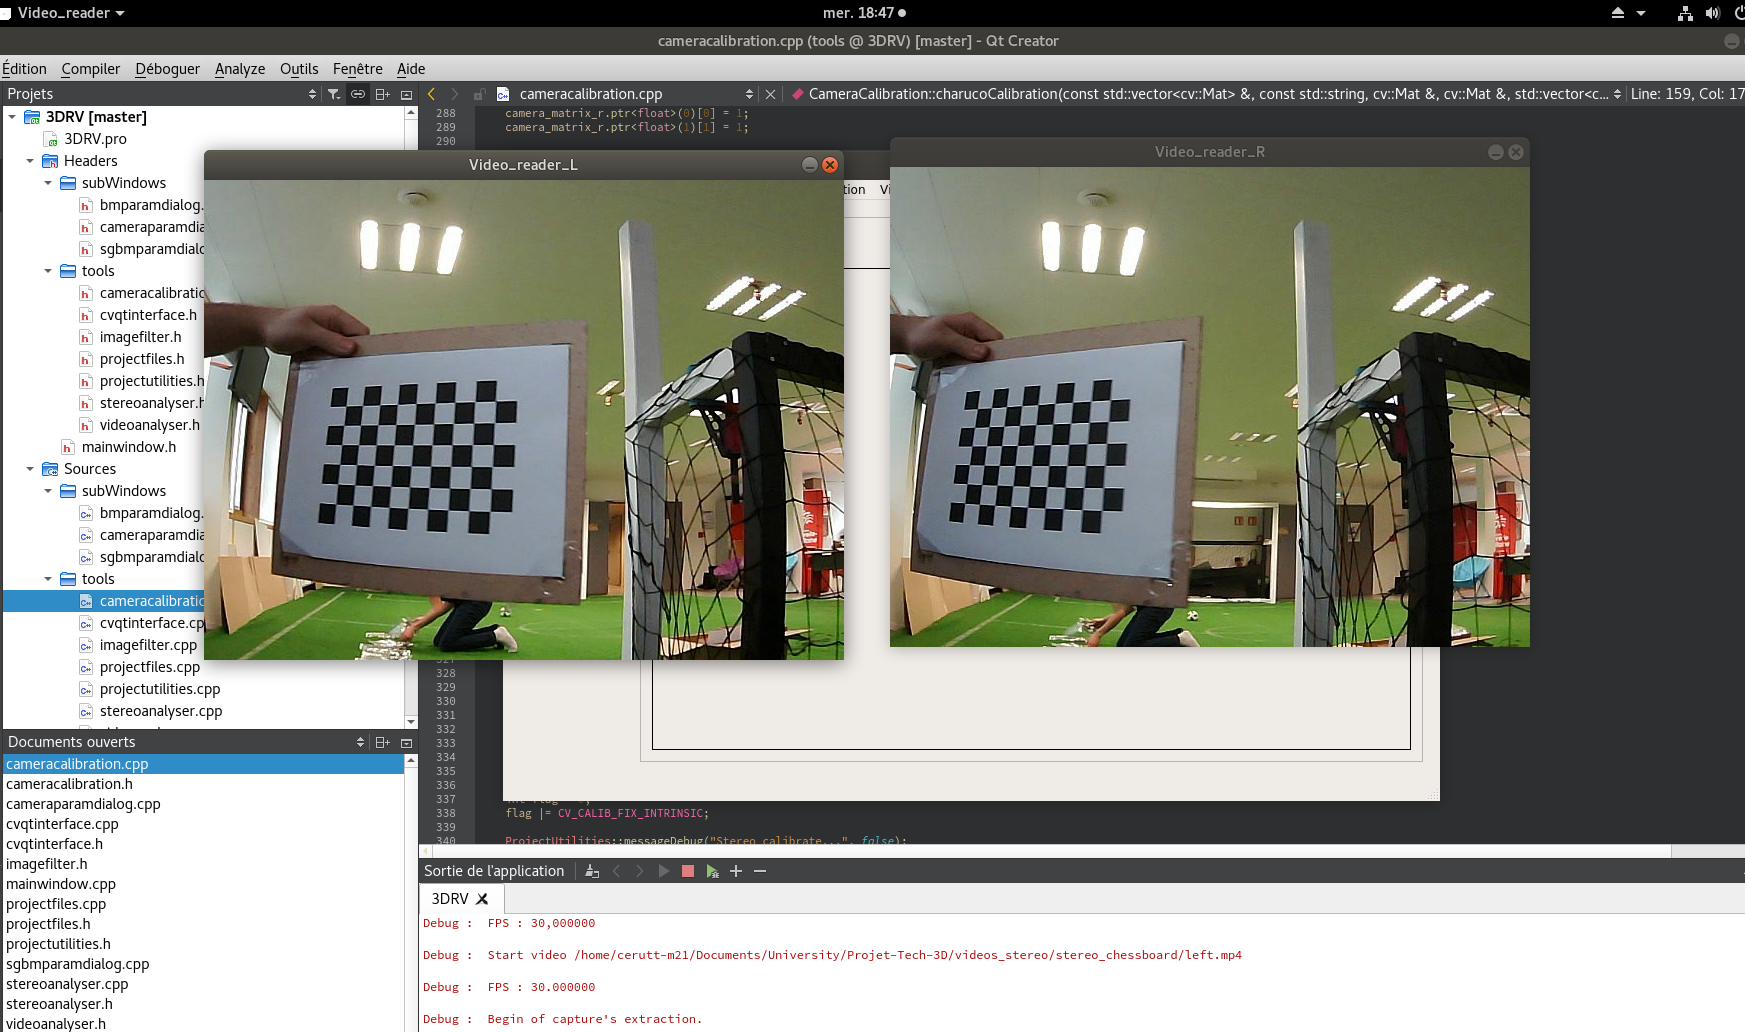
\includegraphics[width=\linewidth]{img/video.png}

Des améliorations devront être fait notamment sur ce dernier point pour pas surchargé la mémoire et pouvoir arrêter en cours de calibration si il s’avère qu'il y a trop d'images.
Un système de choix et de sauvegarde de sets d'images serait aussi appréciable. 

\newpage
\section{Bibliothèque d'analyse}

\subsection{Filtre d'images}

%Photo performances

Ce sont les premières fonctions qui ont été implémenté après l'interface principal. Se sont des fonctions qui seront utilisé plus tard  afin d' analyser les sets d'image que la caméra.

Voici le résultat de chaque :

computeGaussianBlur

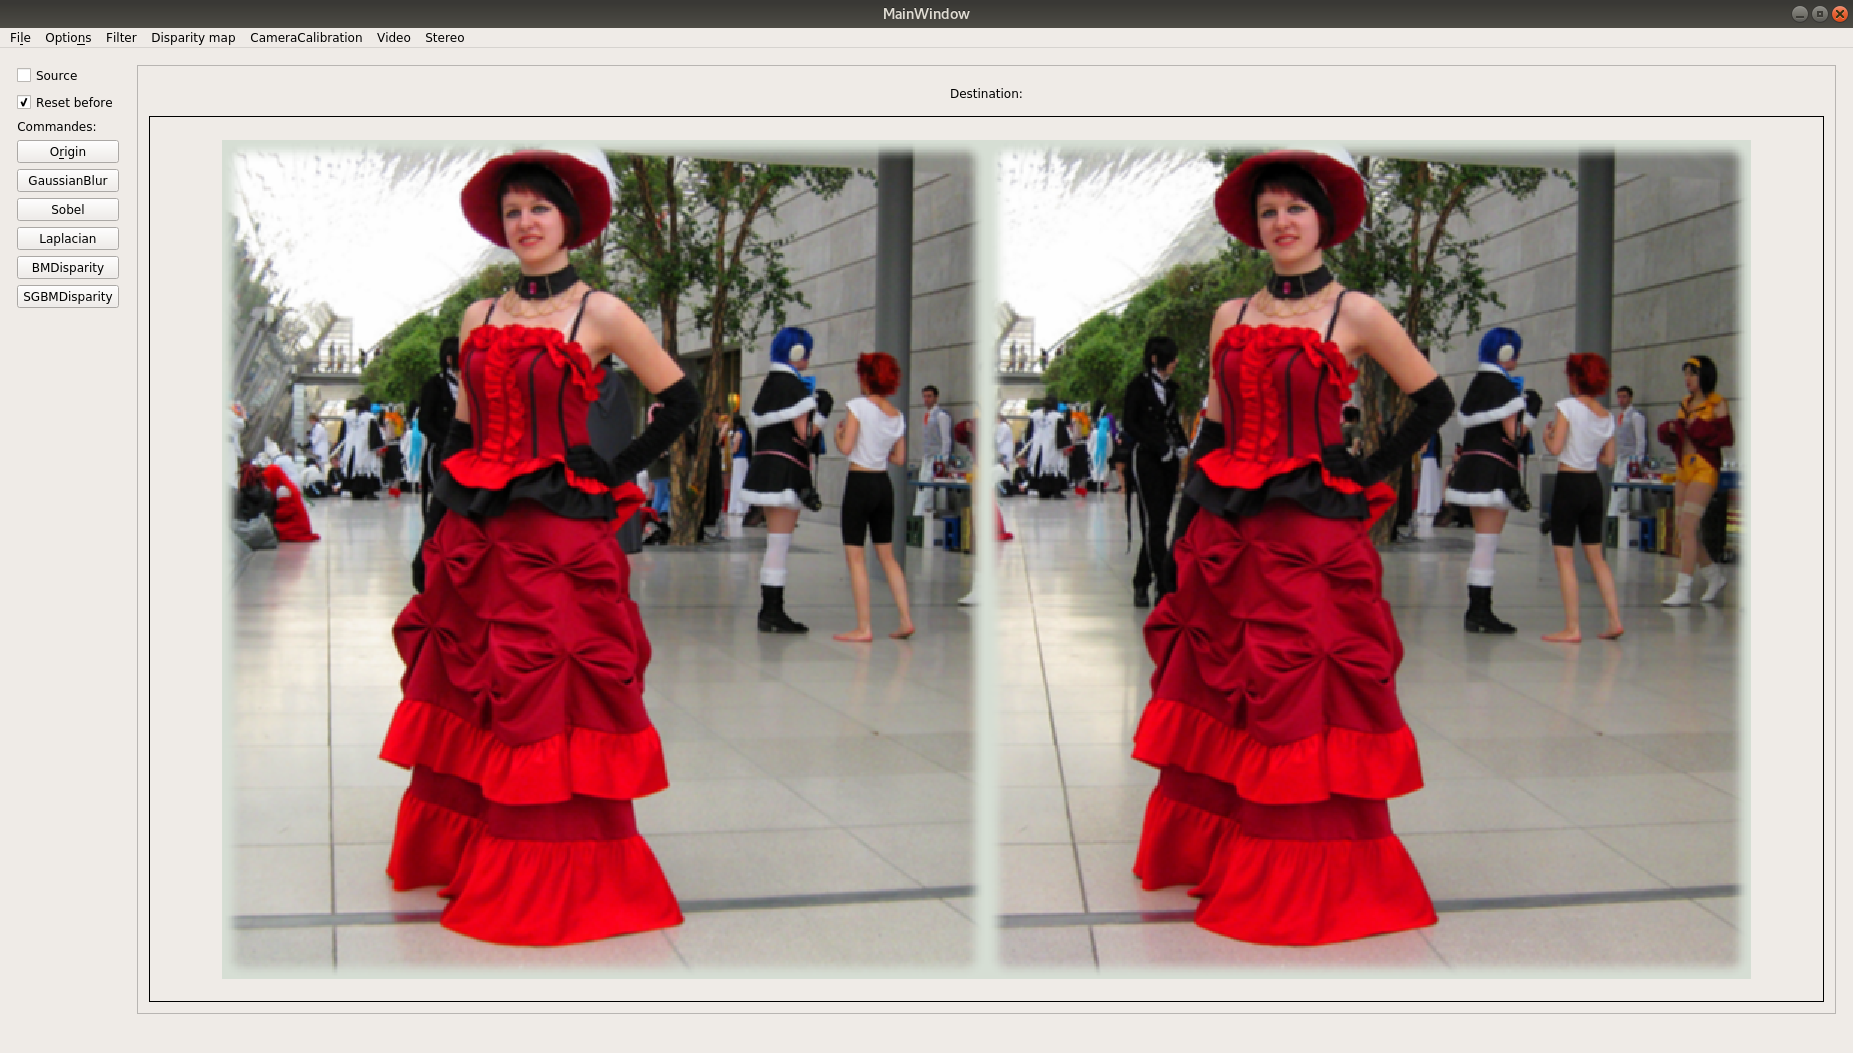
\includegraphics[width=\linewidth]{img/blur.png}

computeGradient

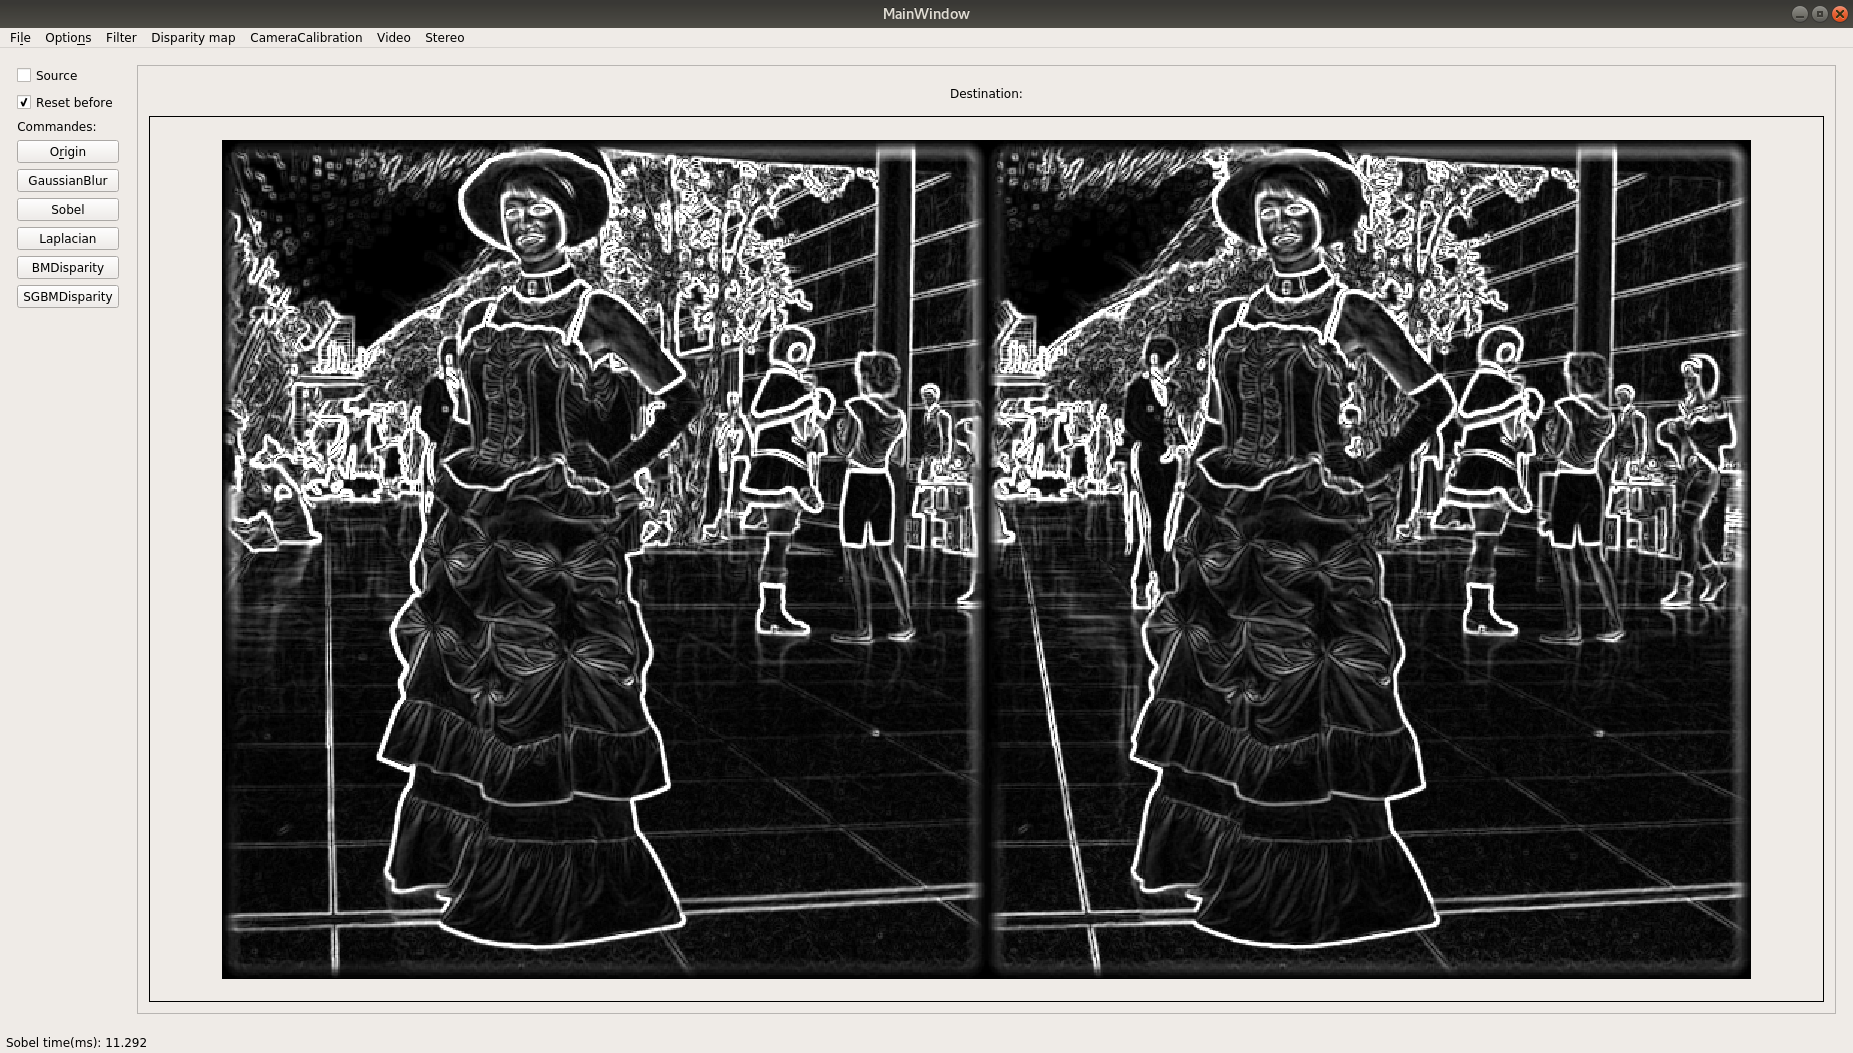
\includegraphics[width=\linewidth]{img/gradient.png}

computeLaplacian

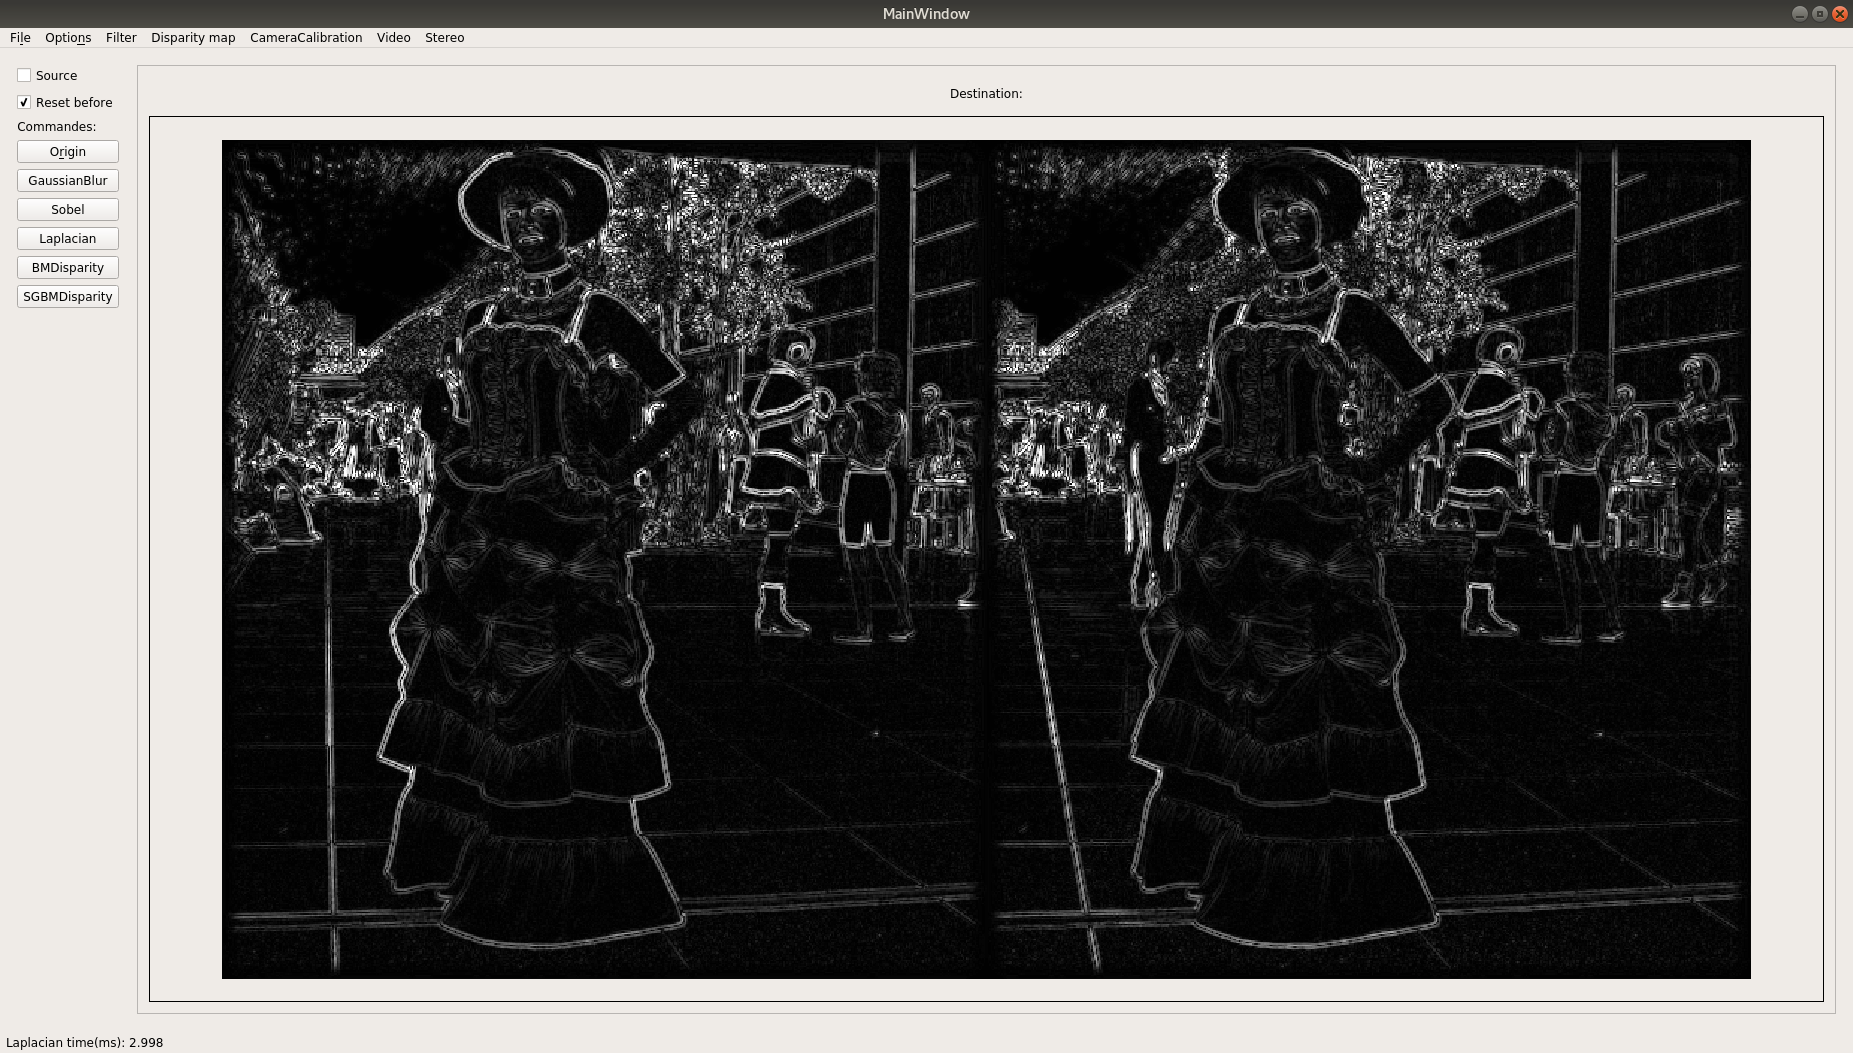
\includegraphics[width=\linewidth]{img/laplacian.png}


\newpage
\subsection{Carte de disparité}

Les cartes de disparité dépendent fortement de paramètres externes à la caméra, la luminosité, la netteté des contours, la focal de la caméra, les couleurs, il devient donc très difficile de choisir les paramètres sans un œil humain, pour avoir un résultat minimal. Il a fallu donc implémenté un système de visualisation pour s'assurer du résultat de ces fonctions.\\

Voici les résultats obtenu avec leur paramètres :

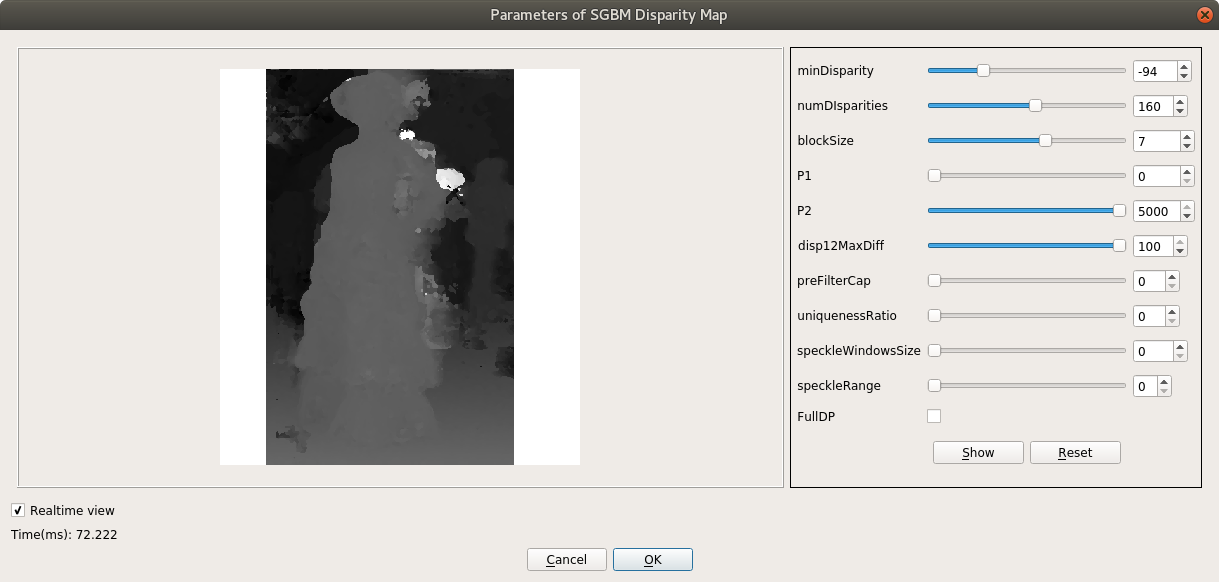
\includegraphics[width=\linewidth]{img/bm.png}

computeBMDisparityStereo
    
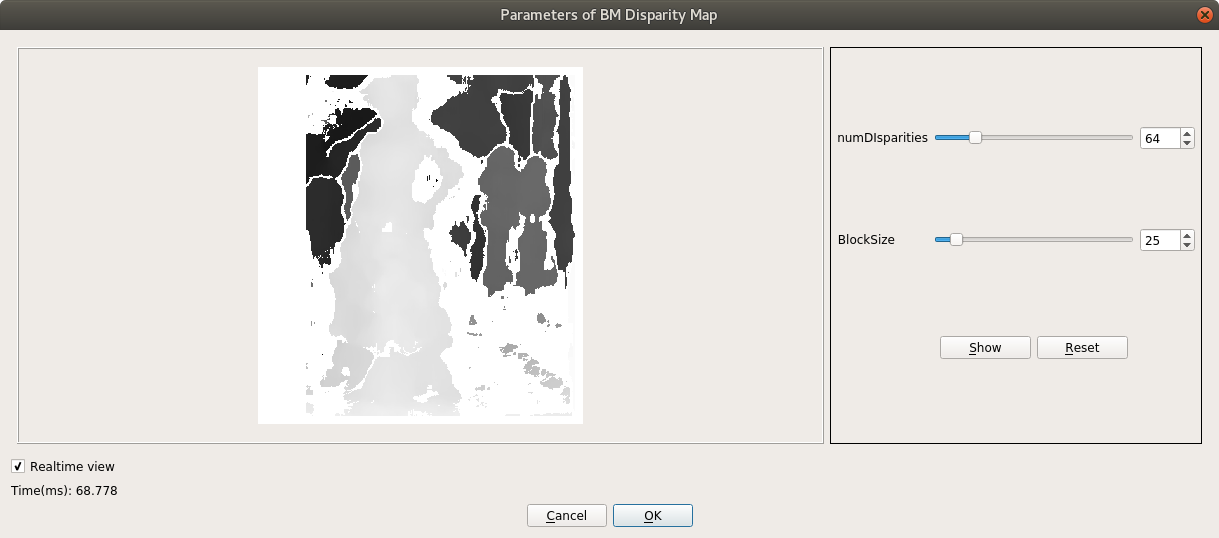
\includegraphics[width=\linewidth]{img/sgbm.png}
    
computeSGBMDisparityStereo

\newpage
\subsection{Calibration Caméra}

%Photo résultat pire-mieux

Pour la calibration, vu les sets d'images qui ont été fourni deux choix s'offrait : la calibration grâce à un damier d'échiquier (chessBoard), et/ou par damier couplé avec un système d'identifiant à la manière des Qr code (Charuco). 
Les deux ont été implémentés avec plus ou moins de succès afin de comparer les résultats.
Avec une grande surprise, les résultats de calibration semble plus prometteur avec le système ChessBoard que Charuco.
Du fait de la distorsion supposé des caméras sans calibration, on peut faire l’hypothèse que l'identification des Id Aruco n'en devient que plus complexe, c'est pourquoi, du fait du manque de temps et aussi de la compatibilité avec la fonction stereoCalibrate de OpenCv, il a été privilégier d'utiliser la solution du ChessBoard plutôt que Charuco, qui même après une première calibration avec ChessBoard, n'affinait pas les résultats et même divergé.

\newpage
\subsection{Analyseur vidéo}

Il a été choisi d'utiliser les fonctions OpenCv pour lire et extraire les frames de la vidéo afin de ne pas surcharger le robot de codes de bibliothèque et aussi pour améliorer les futures performances du robot qui ne demanderait pas d'éventuelles conversion pour une interface graphique.\\

Des problèmes techniques sont néanmoins survenu avec seulement la lecture de vidéo dés le début de l’implémentation de fonctions d'analyse vidéo.\\

Voici d'ailleurs le backtrace reçu avec un segmentation fault.\\

\begin{tabular}{ l l l }

av\_buffer\_unref 									& 							& 0x7fffe0161451 \\
av\_frame\_unref 									& 							& 0x7fffe016d60e \\
??				 									& 							& 0x7ffff27945e8 \\
??													& 							& 0x7ffff27947e0 \\
cvCreateFileCapture\_FFMPEG	 						& 							& 0x7ffff27949f9 \\
?? 													& 							& 0x7ffff279713f \\
cv::VideoCapture::open(cv::String const\&, int) 	& 							& 0x7ffff277e1b0\\
cv::VideoCapture::VideoCapture(cv::String const\&) 	& 							& 0x7ffff277e2be\\
VideoAnalyser::stereoVideoExtraction 				& videoanalyser.cpp(89) 	& 0x5555555910fd\\
MainWindow::on\_actionStereoCalibration\_triggered	& mainwindow.cpp(312)		& 0x555555564589\\
MainWindow::qt\_static\_metacall  					& moc\_mainwindow.cpp(191)	& 0x555555591f87 \\
MainWindow::qt\_metacall  							& moc\_mainwindow.cpp(226) 	& 0x5555555920aa \\
QMetaObject::activate(QObject *, int, int, void * *)& 							& 0x7ffff0b1b784 \\
QAction::triggered(bool)  							& & 0x7ffff13cc1c2 \\
QAction::activate(QAction::ActionEvent) 			& & 0x7ffff13cebb0 \\
??  												& & 0x7ffff153e1ca \\
??  												& & 0x7ffff1545854 \\
QMenu::mouseReleaseEvent(QMouseEvent *) 			& & 0x7ffff1546826 \\
QWidget::event(QEvent *) 							& & 0x7ffff141a278 \\
... <More>      									& & \\                                                                     
 \end{tabular}\\
 
On peut voire ici que sur les machines du Cremi, la bibliothèque FFMPEG est soit mal installé, soit pas à jour. Sachant que sur les machines personnelles, le code marche très bien, et que seul un administrateur peut résoudre ce problème, il a été donc décider de l'ignorer pour l'instant et d'en informer les professeurs.

Ensuite, par manque de temps mais aussi du fait de l'inconnu par rapport au système d'extraction d'image par la caméra, seul les fonctions de Debug et d'extraction furent implémentés, sachant que l'on aurait pu améliorer le code avec une analyse progressive dans une boucle de capture vidéo. 

\newpage
\subsection{Stéréo et carte de profondeur}

    
Pour pouvoir faire la carte de profondeur, il a fallu tout d'abord la calibration de caméra en stéréo.
Cela a nécessité notamment des surcharges de fonctions pour pouvoir directement utiliser deux images au lieu de une seul et de la scinder, par exemple lors de la création de la carte de disparité. Seulement il a fallu aussi faire une fonction spécial de calibration, car l'implémentation à partir de la calibration individuel des caméras devenait beaucoup trop complexe, sachant que les images de calibration devait être mis en rapport et réutilisé lors de la détermination des paramètres extrinsèque en stéréo.
Point de vue performance il y aurait aussi des améliorations à faire sur celle-ci sachant que passé les 40 images, l'attente devient longue (environ 2 min).


Extrait de résultat de calibration stéréo :

Debug :  Calibration finish with left :1.006599 of error. 

Debug :  And right :0.278724 of error. 

Debug :  Calibration finish with 4.994794 of error. 

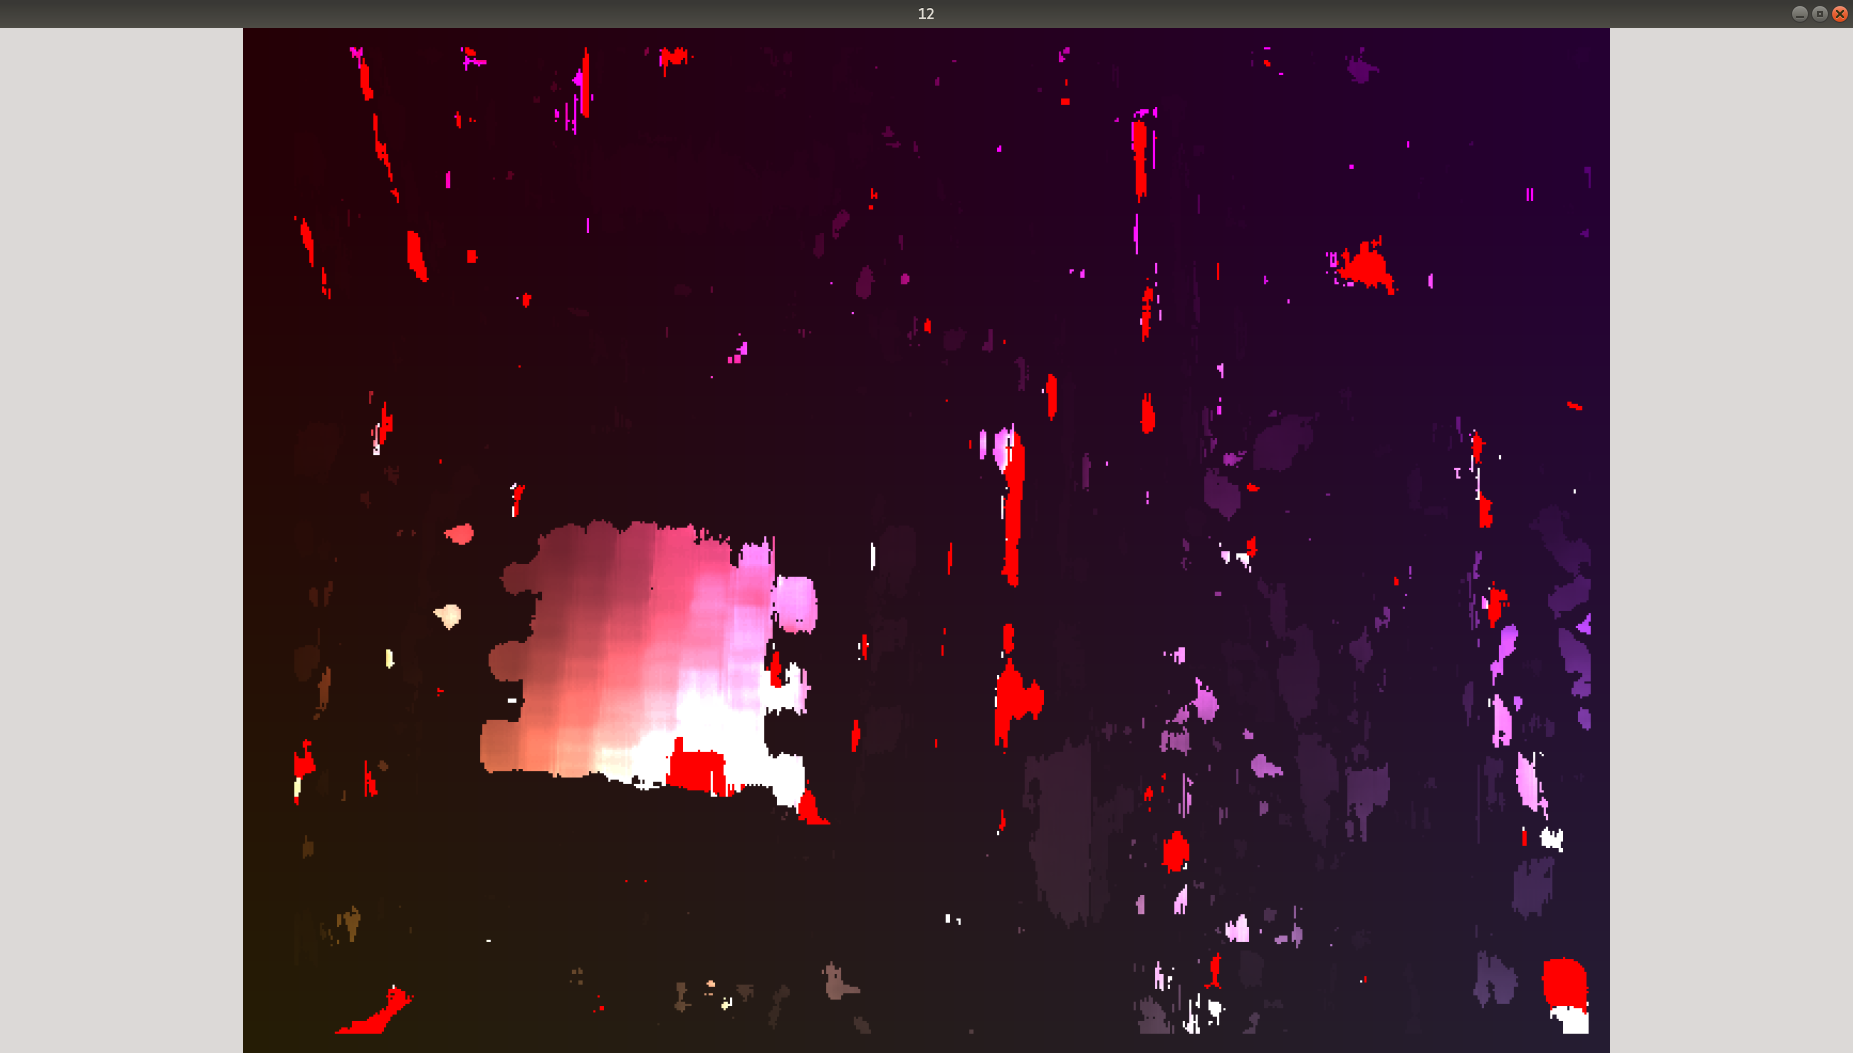
\includegraphics[width=\linewidth]{img/d_bm.png}

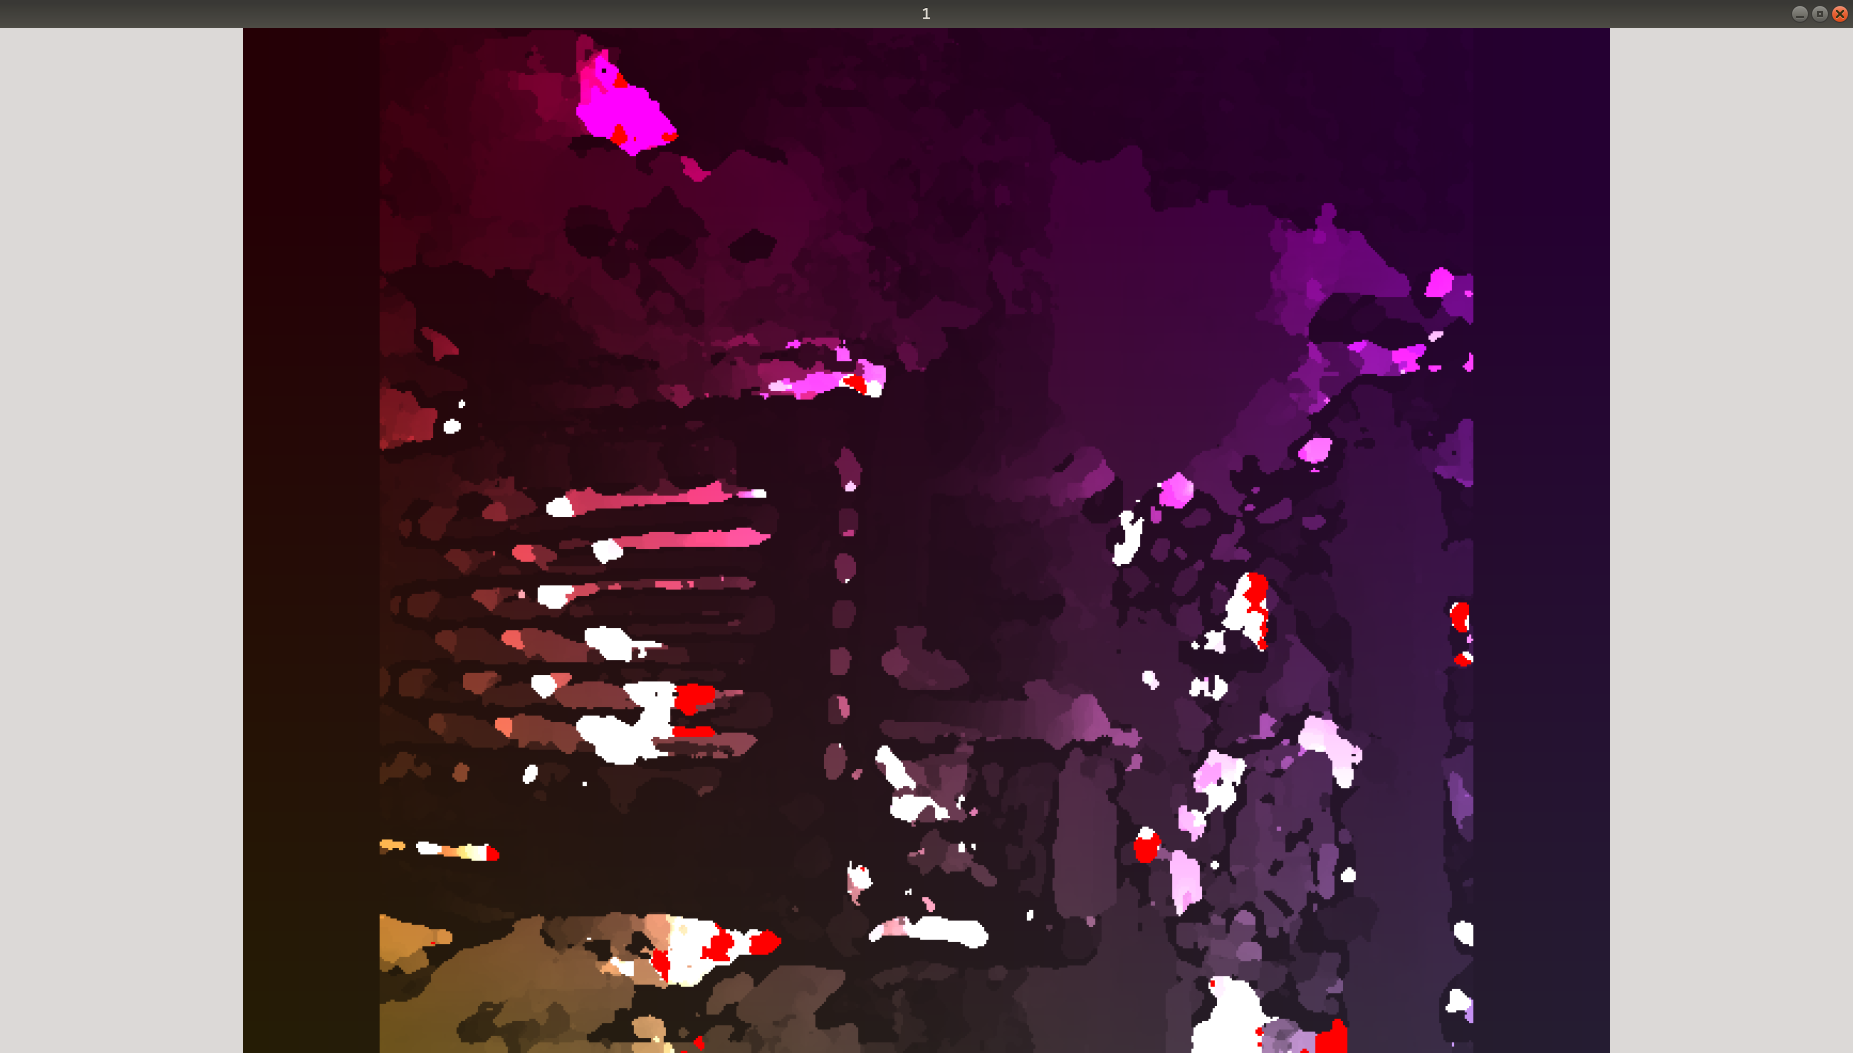
\includegraphics[width=\linewidth]{img/d_sgbm.png}

Ainsi en récupérant les données qu'elle avait produite, et grâce au système d'extraction de vidéo, des résultats ont pu être fourni. 
Une analyse plus poussé des résultats sont cependant nécessaires pour analyser extraire les points sur un repère 3D.

    \newpage
\subsection{Fichiers et sauvegarde}

Basé sur le système déjà existant de FileStorage d'OpenCv, les calibration mono et stéréo ont été sauvegardé en format XML, du fait de l'utilisation répandu de celui-ci.
Les fichiers sauvegardé et utilisé plus haut sont d'ailleurs en annexe.

%------------------%
    
\begin{comment}
\newpage
\section{Simulation}
\end{comment}

%------------------%
\begin{comment}
\newpage
\part{Tests}

\section{Tests unitaires}

\section{Performances}

\subsection{Filtre d'images}

%Tableau performances

\subsection{Carte de disparité}

%Tableau performances

\subsection{Calibration Caméra}

%Tableau performances

\subsection{Carte de profondeur}

%Tableau performances
\end{comment}

%------------------%
\newpage
\part{Bilan}

\section{Semestre 5}

\subsection{Difficultés rencontrés}

Les difficultés rencontré ont été diverses. Du fait déjà que j'ai été seul sur le projet, la recherche de documentation s'en retrouvé plus difficile et la productivité en était plus réduite surtout sur les interfaces qui était secondaire par rapport à la qualité d'analyse. Cette même qualité notamment sur les cartes de disparité et la calibration était très difficile à atteindre du fait de paramètres optionnels dans OpenCv, mais néanmoins important. Parfois même, c'était difficile de savoir ce que l'on attendait comme résultat. Mais grâce au dialogue et à la comparaison de résultat avec d'autres groupes, ces dernières difficultés ont en parti été surmontés.

\subsection{Critique et améliorations potentielles}

L'amélioration de l'interface pour la vidéo et les cartes de profondeur améliorerait la visualisation des résultats. Plus que une amélioration du système de base, ce qu'il faut est une refonte pour pouvoir accueillir la visualisation de stéréo, ce qui n'a pas forcément été bien pris en compte dès le début du projet du fait des images stéréo rassemblé en une seul image.
Il manque d'ailleurs les performances pour la carte de profondeur et la calibration, il y a aussi une incohérence avec les couleurs lors du choix de la carte de disparité sur computeDepthMap.

\begin{comment}
\section{Semestre 6}
\subsection{Difficultés rencontrés}
\subsection{Critique et améliorations potentielles}
\end{comment}

%------------------%
\newpage
\appendix
\part{Annexes}

\listoffigures

\newpage
\section{Hiérarchie du projet}
\lstinputlisting[]{hierarchie.txt}

\newpage
\section{Files}

\subsection{Left calibration}

\lstinputlisting{results/l_calibration.xml}

\newpage
\subsection{Right calibration}

\lstinputlisting{results/r_calibration.xml}

\newpage
\subsection{Stereo calibration}

\lstinputlisting{results/stereo_calibration.xml}

\newpage
\section{Rapports}
\subsection{Rapport Initial}
Scission du groupe initial du fait de problèmes internes concernant des choix d'implémentation de l'interface graphique.\\

Fonctionnalités de base déjà présentes à ce moment :\\
	-Fonctions de conversion basique d'images de OpenCv vers Qt.\\
	-Mise en place d'une bibliothèque graphique d'analyse adaptant les fonctions d'OpenCv.\\
	-Ouverture de dialogues particulier pour les cartes de disparité.\\
	-Filtres de flou Gaussien, de Laplacien, et de séparation d'image pour les cartes de disparité implémenté.\\
	-Fonction de débogage d'image pour l'affichage OpenCv crée.\\


\subsection{Rapport 05 novembre 2018}

\textbf{Rapport du groupe CERUTTI}\\
Le 05 novembre 2018\\

Interface graphique:\\
	-Rajout d'une check box pour remettre à l'image d'origine automatiquement dans la fenêtre principal.\\
	-Rajout de l'affichage de l'approximation de l'efficacité des fonctions.\\
	-Mise a jour du code des boutons, des menus, et des fenêtres pour implémenter ces nouvelles mécaniques.\\
	-Rajout d'une fenêtre pour les paramètres de StereoBM.\\
	-Rajout des boutons de Sobel et Flou gaussien.
\\
	
Analyse d'images:\\
	-Amélioration des algorithmes pour prendre en charge les images en GrayScale, permet d'enlever les conversions redondantes, et l'utilisation des fonctions de manière successives facilité.\\
	-Rajout de showMatrice(cv::Mat mat) dans ImageAnalyser pour le débuguage.\\
	-Rajout de computeEfficiency(double time, func, args) pour avoir une approximation de l'efficacité des algorithmes.\\
	-Rajout des fonctions Sobel et Flou gaussien.\\

Mise en place d'un exécutable pour les tests d'analyse d'images.\\

Pistes d'améliorations:\\
	-Implémentation des tests\\
	-Recherche des meilleurs paramètres pour algorithmes stereo\\
	-Factorisation du code pour les fenêtres BM et SGBM\\
	-Recherche sur la possible utilisation de threads\\
	-SteroVar non essayé openCv\\
	-Recherche analyse de flux vidéo\\
	-Recherche object tracking et template
\\

\textbf{Remarques professeur :}\\
Pas d'image dans Git\\
Signaler fuites mémoire, même bibliothèque\\
Sobel demandé n'est pas juste l'utilisation la fonction de OpenCv, l'objectif était de faire un gradient\\
Voire problème de carte de disparité\\
Trop de découpage  de code\\
Laisser le code cvtColor dans les fonctions nécessaires sinon cela ne facilite pas la lecture de code\\
Mettre des références à la place de la recopie de matrice
\\\\

\textbf{Prochain rapport :}\\
Simplifier le code\\
Renommer les variables avec convention (code et fichiers) et commenter le code\\
Voire carte disparité problème\\
Prévoir quoi faire avec le matériel\\
Calibration\\
\\

\subsection{Rapport 5 Décembre 2018}
Rapport du groupe CERUTTI
Le 05 Décembre 2018


Correction depuis dernier rendu:

    -Adoption d'une convention de nommage:\\
\begin{tabular}{ l c }
   Attribut & \textit{\_name\_complete }\\
   Variables locales  & \textit{name\_complete}\\ 
   Méthodes & \textit{nameComplete}\\
   Classes 	& \textit{NameClass}\\
   Fichiers	& \textit{nameclass.*}\\
 \end{tabular}\\
 
    -Changement de la fonction Sobel en Gradient, et implémentation en vrai Gradient.\\
    -Correction des cartes de disparité inversé\\
    -Amélioration des performances en enlevant la recopie des return et en passant des références en paramètre.\\
   

Calibration:\\
    -Implémentation de findOneCalibration. Pour une image particulier il trouve les paramètres de calibration, et les mets dans un fichier. Il envoie ensuite dans la matrice de sortie l'image non distordue.\\
    -Test valgrind, 32 erreurs externes (supposé lié à la bibliothèque Qt)\\

Interface graphique:\\
    -Rajout d'une option TestCameraCalibrate, dans les menus prend l'image courant d'interface et applique findOneCalibration.\\
Remarque, certaines images sont distordus comme la set1/10\_20\_43\_159.jpg après calibration. Possibilité que le ChessBoard soit trop loin, couplé au fait qu'il n'y a qu'une seule valuation de calibration.
\\

Pistes d'améliorations:\\
    -Filtre pour les cartes de disparité (si cela n'impacte pas les performances)\\
    -Créer un système de sauvegarde général pour calibration et performances.\\
    -Améliorer le système de calibration par multiples valeurs et prise en charge automatique de calibration par dossier d'images.\\
    -Améliorer l'interface pour prendre en compte la calibration de différentes caméras.\\

\textbf{Remarques professeur :}\\
-Sobel erreur\\
-Synthèses à améliorer\\
-enlever qtdesigner.txt\\
-mettre algos\\
-résultats\\
-problème\\
-pas de code dans rapport\\
-Erreur récurrentes (?)\\
-Rigueur sur le code, moins sur la théorie\\
-Rapport pas un bilan d'activité\\
\\

\textbf{Prochain rapport :}\\
Faire un deuxième système de calibration par ChAruco.\\
Calculer cartes de profondeur.\\
Rendu du rapport de semestre 5\\
Implémenter des tests unitaires et de performances.\\
Améliorer l'interface pour prendre en compte l'affichage de calibration.\\
(Filtre pour les cartes de disparité)\\
\\\\


\end{document}
